\section{Tecnologie implementate}
Conclusa la spiegazione della modellazione dei link e della vite è il momento di iniziare l'attività sperimentale. Lo scopo di questa sezione è l'introduzione alle tecnologie software utilizzate per la modellazione reale del manipolatore.
\subsection{Simulink Real time}
Simulink \textit{real-time} è un plugin di matlab, consente di creare applicazioni real-time ed eseguirle su un hardware target, come per esempio un computer. Simulink-real time gira su un computer di "sviluppo" che è il PC utente, ed è diverso dal sistema che permette il movimento e l'esecuzione del modello in tempo reale ovvero il dispositivo target. Grazie a questo il software permette raggiungere tempi di campionamento molto più veloci per uno stesso modello (vi è la possibilità di raggiungere frequenze fino a 20 kHz) rispetto ad \textit{kernel real-time} che condivide le risorse hardware con il computer.
Un'altra caratteristica fondamentale è il fatto che su SLRT è possibile far funzionare il dispositivo target in modalità \textit{stand-alone}, si può riuscire a far avviare il dispositivo senza il bisogno di una vera e propria procedura d'installazione.

\subsection{EtherCAT}
L'obiettivo di questa sottosezione è quello di presentare il protocollo di comunicazione utilizzato per interfacciarsi col robot PKM, evidenziandone le sue caratteristiche principali.
\par EtherCAT è una tecnologia ethernet sviluppata ed introdotta nell'aprile 2003 da Beckhoff automation. Il protocollo è stato pubblicato nello standard IEC61158, e regolato dalla società ETG (\textit{EtherCAT Technology Group}), soddisfa i requisiti \textit{hard} e \textit{soft} real time specifici per l'ambito dell'automazione. Una caratteristica molto nota riguarda la velocità dei tempi di ciclo, la durata media di un periodo di ciclo è inferiore a $100 \mu s$. 
\subsubsection{Proprietà}
%\addcontentsline{toc}{subsubsection}{Proprietà}
 Il principio base di funzionamento di EtherCAT si basa sul concetto di \textit{Master/Slave}. Il master invia un pacchetto, chiamato telegramma che va ad attraversare tutti i nodi, ogni singolo slave collegato legge i dati che riguardano lui e scrive i dati prodotti intanto che il telegramma si propaga sulla rete verso i nodi successivi. Non appena il pacchetto arriva all'ultimo nodo, è quest'ultimo che si occupa di reinviarlo al master grazie alla comunicazione \textit{full-duplex} presa da Ethernet, facendo questo, il flusso di dati teorico riesce a superare i $100 Mbit/s$. \par Il fatto che il master sia l'unico nodo che può inviare frame in maniera attiva garantisce prestazioni deterministiche; inoltre, utilizza un Media Access Controller (MAC) standard, senza alcun processore dedicato alla comunicazione. Questo consente di implementare un dispositivo master su una qualunque piattaforma hardware dotata di una porta di rete, indipendentemente dal sistema operativo o dal software applicativo utilizzato. I dispositivi EtherCAT slave integrano un EtherCAT \textit{Slave Controller} (ESC) in grado di processare i frame \textit{on-the-fly} e in modo puramente hardware, il che rende le prestazioni della rete predicibili e indipendenti dalla particolare implementazione dei dispositivi slave.
\subsubsection{Gestione della rete}
Caratteristica fondamentale della rete è la sicurezza, viene implementata una tecnologia denominata \textit{safety over EtherCAT} che consente la realizzazione di architetture di sicurezza più semplici e flessibili di una logica standard a relè. Vi è la possibilità di trovare questa tecnologia standardizzata nella specifica IEC 61784-3, il sistema di comunicazione è parte del \textit{black channel}, ovvero una sezione considerata non rilevante ai fini della sicurezza; viene utilizzato un solo canale per trasferire sia i dati standard che quelli di sicurezza, in particolare i frame di sicurezza vengono identificati come \textit{safety container}, e contengono i dati critici del processo e l'informazione necessaria per garantirne l'integrità. Il \textit{safety container} viene mappato dentro i dati di processo che sono ciclici durante la comunicazione; possono viaggiare tramite cavi di rame, fibre ottiche e connessioni wireless. La variabilità del mezzo trasmissivo introduce flessibilità, e rende più semplice e sicura la connessione tra parti della macchina anche lontane fra di loro. In una macchina completamente connessa, andare ad implementare una funzione d'arresto di emergenza totale risulterà semplice anche se altre parti della macchina sono connesse mediante tecnologie diverse. 
\subsubsection{Implementazione interfacce}
Come abbiamo accennato precedentemente, il principio di funzionamento di \textit{EtherCAT} è il concetto di \textit{master/slave}; per come si è evoluta questa tecnologia, e considerando che l'interfaccia non richiede una CPU ad elevate prestazioni, è possibile andare ad aggiungere un dispositivo di I/O ad un controllore senza andare ad aumentare significativamente i costi complessivi. Per un cliente, è importante l'interoperabilità tra i dispositivi di più fornitori, per questo prima di poter introdurre un dispositivo sul mercato vengono fatti tutti i test, che verificano che l'implementazione rispetti la specifica EtherCAT.
\par L'interfaccia master ha l'unico requisito di avere una porta ethernet, per l'implementazione viene utilizzato o l'ethernet controller integrato oppure una schede di rete base; nella maggior parte dei casi l'\textit{ethernet controller} viene integrato mediante un DMA (\textit{Direct Memory Access}), in questo modo per l'invio dei dati tra il master e la rete non vengono utilizzate le risorse della CPU. Gli slave scrivono i dati prodotti e leggono quelli a loro indirizzati mentre il telegramma li attraversa, facendo così al master arriva l'immagine già ordinata correttamente, la CPU quindi non è più responsabile dell'ordinamento. I dispositivi \textit{slave} invece utilizzano l'ESC (\textit{Ethercat slave controller)}, solitamente di costo contenuto oppure integrato in un microcontrollore standard, esistono slave semplici che non richiedono nemmeno la presenza di un microcontrollore per il fatto che gli ingressi e le uscite digitali possono essere direttamente collegati all'ESC, mentre per quelli più complessi viene usato un controllore a 8-bit.
\subsection{CME2}
CME2 è un software prodotto da Copley control, e serve per la configurazione degli azionamenti. Le funzioni principali riguardano \textit{auto-phasing} e \textit{auto-tuning}, che vanno a semplificare la realizzazione del sistema. Oltre a queste due funzioni principali abbiamo anche le tabelle Cam che forniscono un buon approccio per la produzione di movimenti sincronizzati e ripetitivi ad un dispositivo esterno, e la possibilità di definire sequenze fino a 32 indici oppure indicizzate. Sono anche predisposte funzioni per l'analisi degli strumenti, la configurazione dei motori dei filtri e dei guadagni, è possibile anche andare a cambiare la modalità operativa, scegliendo quindi se lavorare con un anello in posizione, corrente o coppia. Il collegamento con gli azionamenti avviene tramite cavo ethernet
\begin{figure}[ht]
\begin{center}
    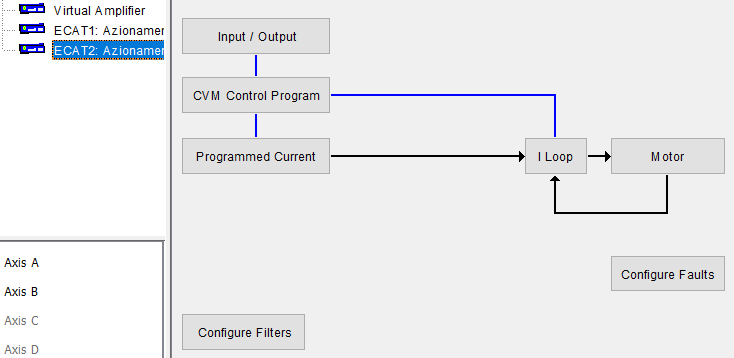
\includegraphics[scale=0.8]{Immagini/Sperimentale/azionamenti.PNG}
    \caption{Schema azionamento}
\end{center}
\end{figure}
\\come si può notare dalle foto gli azionamenti sono controllati in coppia, in particolare viene chiuso l'anello in corrente grazie ai parametri del motore. Un'operazione fondamentale è stata l'analisi dei registri alla ricerca di quelli dei finecorsa\footnote{Il registro del finecorsa passa da \textit{LOW} a \textit{HIGH} dopo che il manipolatore lo raggiunge.}
Per le braccia, i registri da guardare sono l'ottavo e il quindicesimo, in particolare per vincoli di progetto i finecorsa osservati sono stati quelli al lato destro, quindi quando le braccia sono entrambe a destra; per la vite invece il registro osservato è stato il quindicesimo, riferito a quando la vite arriva a toccare il lato superiore.
\begin{figure}[ht]
\begin{center}
    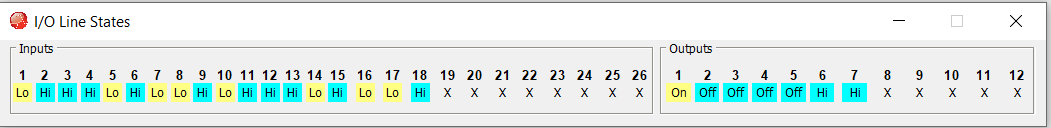
\includegraphics[scale=0.6]{Immagini/Sperimentale/registri.PNG}
    \caption{Registri azionamento}
\end{center}
\end{figure}
\subsection{EC-Engineer}
EC-Engineer è uno strumento software utilizzato per la configurazione, diagnostica e monitoraggio delle reti EtherCAT, è nato con lo scopo di aver tutto il necessario su un solo ambiente. Usando questo programma è possibile generare due tipologie di configurazioni EtherCAT, online oppure offline. Il primo tipo di configurazione viene fatto quando siamo direttamente connessi sulla macchina alla rete EtherCAT quindi è un'operazione fatta in real-time, la seconda tipologia invece può essere fatta in laboratorio o ufficio e non richiede la connessione alla rete in quel preciso momento. Per andare a fare una connessione online non è necessario che gli slave siano direttamente connessi al PC locale, questo grazie alla funzione \textit{bus scan} che permette di andare a determinare la topologia della rete facilmente. Nel nostro caso la configurazione è stata fatta \textit{offline}, e come metodo di comunicazione si è scelto di usare le PDO\footnote{\textit{Process Data Object}, ovvero dati trasmetti dal/al \textit{MotionController}, in tempo reale a tutti i nodi ogni ciclo del tempo di campionamento.}. L'ulotimo passo della configurazione è l'esportazione di un file ENI, un file XML che descrive la topologia della rete specificando il comando di inizializzazione per ogni dispositivo ed i comandi che devono essere inviati ciclicamente.
